\clearpage
\begin{nquote}{}
	``*chuckles* I'm sorry, but all of this seems obvious." - Dr. Loewen, 11/3/2023
\end{nquote}

\subsection{Neighbourhoods and interiors}
\begin{ndef}{: Neighbourhood}
	Given a HTS  \((\mc{X},\ms{T})\) and an \(x\in\mc{X}\), a set \(\mc{S}\subseteq\mc{X}\) is a \emph{\textbf{neighbourhood}} of \(x\) exactly when there exists \(\mc{U}\subseteq\ms{T}\) such that \(x\in\mc{U}\subseteq\mc{S}\). We write \(\ms{N}(x)\) to be the set of all such \(\mc{S}\).
\end{ndef}
\begin{figure}[htbp]
	\centering
	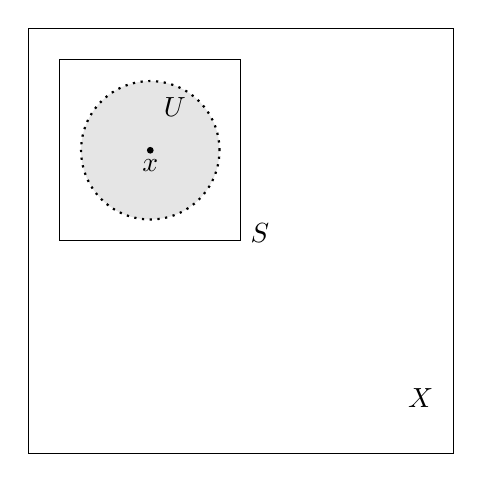
\begin{tikzpicture}
		\draw[] (2.7, 2.7) -- (-2.7, 2.7) -- (-2.7, -2.7) -- (2.7, -2.7) -- (2.7, 2.7);
		\draw[] (-2.3, 0) -- (-2.3, 2.3) -- (0, 2.3) -- (0, 0) -- (-2.3, 0);
		\draw[dotted, thick, fill = white!60!lightgray] (-1.15, 1.15) circle (25pt);
		\draw[fill] (-1.15, 1.15) circle (1pt);
		\node[below] at (-1.15, 1.15) {\(x\)};
		\node[right] at (-1.1, 1.7) {\(\mc{U}\)};
		\node[right] at (2, -2) {\(\mc{X}\)};
		\node[right] at (0, 0.1) {\(\mc{S}\)};
	\end{tikzpicture}
	\caption{Visualization of the definition.}
\end{figure}
\begin{nlemma}{}
	In any HTS \((\mc{X},\ms{T})\) with \(\mc{A}\subseteq\mc{X}\), the following are equivalent:
	\begin{enumerate}[(a)]
		\item \(\mc{A}\) is open.
		
		
		\item For all \(x\in\mc{A}\), we have \(\mc{A}\in\ms{N}(x)\).
	\end{enumerate}
\end{nlemma}
\begin{proof}[Proof sketch]
	Just pushing around definitions, nothing too complex.
\end{proof}
\begin{ndef}{: Interior points}
	In a HTS \((\mc{X},\ms{T})\) with \(\mc{A}\subseteq\mc{X}\), a point \(x\) is an \emph{\textbf{interior point of \(\mc{A}\)}} if there exists \(\mc{U}\in\ms{N}(x)\) such that \(\mc{U}\subseteq\mc{A}\).
	
	\medskip
	
	The collection of interior points is
	\begin{equation*}
		\mc{A}^{\circ}=~\text{``the interior of \(\mc{A}\)."}
	\end{equation*}
\end{ndef}
\begin{note}
	If \(\mc{A}\subseteq\mc{B}\), then \(\mc{A}^{\circ}\subseteq\mc{B}^{\circ}\).
\end{note}
\begin{nproposition}{}
	In a HTS \((\mc{X},\ms{T})\) with \(\mc{A}\subseteq\mc{X}\),
	\begin{enumerate}[(a)]
		\item \(\mc{A}^{\circ}\) is \emph{open}, with \(\mc{A}^{\circ}\subseteq\mc{A}\).
		
		\item If \(\mc{G}\) is open, and \(\mc{G}\subseteq\mc{A}\), then \(\mc{G}\subseteq\mc{A}^{\circ}\); \(\mc{A}^{\circ}\) is the \textbf{largest open subset} of \(\mc{A}\).
		
		\item \(\mc{A}\) is open iff \(\mc{A}=\mc{A}^{\circ}\).
	\end{enumerate}
\end{nproposition}
\begin{proof}
	The proofs for these are very short and given in the notes, but the professor suggested we try to do them ourselves.
\end{proof}
\begin{note}
	The shape of our neighbourhood depends on the topology we lay down on the space; if we look at the real line, the topology on it \emph{does not} allow a point to be its \emph{own} neighbourhood.
\end{note}
\begin{example}
	If \(a<b\) in \(\R\), we have 
	\begin{equation*}
		[a,b]^{\circ}=[a,b)^{\circ}=(a,b]^{\circ}=(a,b)^{\circ}=(a,b).
	\end{equation*}
	Observe that \(\Q^{\circ}=\emptyset\).
\end{example}
\begin{note}
	The ``largest open subset" is as shown above, and the ``smallest open subset" does not exist. We illustrate this in \(\R\) as follows: Consider \(\mc{A}=[0,1]\); If \(\mc{U}\) is open, and \(\mc{U}\supset\mc{A}\), then \(0\in\mc{U}\) and \(1\in\mc{U}\) imply that there exists a sufficiently large \(n\in\N\) such that \(\left(-\displaystyle\frac{1}{n},\frac{1}{n}\right)=\displaystyle\B\left[0;\frac{1}{n}\right)\subseteq\mc{U}\) and \(\left(1-\displaystyle\frac{1}{n},1+\frac{1}{n}\right)=\displaystyle\B\left[1;\frac{1}{n}\right)\subseteq\mc{U}\). So, \(\mc{U}\supseteq\left(\displaystyle-\frac{1}{n},1+\displaystyle\frac{1}{n}\right)\). Increasing \(n\) gives us a smaller alternative that is still open and covers \([0,1]\); no smallest such subset exists.
	\begin{equation*}
		\bigcap_{n=1}^{\infty}\left(-\frac{1}{n},1+\frac{1}{n}\right)=[0,1].
	\end{equation*}
\end{note}
\subsection{Closed sets; Closure}
\begin{ndef}{: Closed set}
	In a HTS \((\mc{X},\ms{T})\), a set \(\mc{F}\subseteq\mc{X}\) is \emph{\textbf{closed}} iff \(\mc{F}^c=\mc{X}\backslash\mc{F}\) is open.
\end{ndef}
Imagine defining \(\ms{F}:=\{\mc{U}^c:\mc{U}\in\mc{J}\}\) is the set of all closed subsets in \(\mc{X}\). The HTS axioms could be set up starting with closed sets and \(\ms{F}\) instead of open sets and \(\ms{T}\), and this would be logically equivalent:
\begin{enumerate}[(HTS~1)]
	\item \(\emptyset,\mc{X}\in\ms{F}\); note that these sets are both closed and open (by definition). These can also be called ``clopen" sets.
	
	\item Arbitrary intersection of closed sets is closed: if \(\ms{K}\subseteq\ms{F}\) then \(\displaystyle\bigcap\ms{K}\in\ms{F}\), where 
	\begin{align*}
		\bigcap\ms{K}=&\bigcap_{\mc{K}\in\ms{K}}\mc{K}\\
		=&\left(\bigcup_{k\in\ms{K}}\mc{K}^c\right)^c.
	\end{align*}
	
	\item If \(\mc{F}_1,\dots,\mc{F}_N\) are closed are closed (where \(N\in\N\)), then \(\displaystyle\bigcup_{j=1}^N \mc{F}_j\) is closed as well, where 
	\begin{equation*}
		\left(\bigcup_{j=1}^N \mc{F}_j\right)^c=\bigcap_{j=1}^N(\mc{F}_j^c)\in\ms{T}.
	\end{equation*}
	
	\item If \(x_1\neq x_2\) in  \(\mc{X}\), there exist \(\mc{F}_1,\mc{F}_2\in\ms{F}\) such that \(x_1\notin\mc{F}_1\), \(x_2\notin\mc{F}_2\), \(\mc{F}_1\cup\mc{F}_2=\mc{X}\).
\end{enumerate}
\begin{note}
	As HTS 1 already suggests, if a set is not open, it \emph{\textbf{does not}} mean it is closed; it could be clopen, which is purely a definition. This is also why I think the names are not good because ``sets are not doors" - Dr. Jim Bryan, 2023.
\end{note}
\begin{ndef}{: Closure}
	In a HTS \((\mc{X},\ms{T})\) with \(\mc{A}\subseteq\mc{X}\), the \emph{\textbf{closure}} of \(\mc{A}\) is the set 
	\begin{equation*}
		\ol{\mc{A}}:=\left(\left(\mc{A}^c\right)^{\circ}\right)^c,
	\end{equation*}
	which is the complement of an open set \(\left(\left(\mc{A}^c\right)^{\circ}\right)\), so it is closed:
	\begin{align*}
		&(\mc{A}^c)^{\circ}\subseteq\mc{A}^c\\
		\implies &\left(\left(\mc{A}^c\right)^{\circ}\right)^c\supseteq \left(\mc{A}^c\right)^c=\mc{A}\\
		\implies& \ol{\mc{A}}\supseteq\mc{A}.
	\end{align*}
\end{ndef}
Indeed \(\ol{\mc{A}}\) is the smallest closed superset of \(\mc{A}\); if \(\mc{F}\) is closed, and \(\mc{F}\supseteq\mc{A}\), then \(\mc{F}\supseteq\ol{\mc{A}}\) as well.
\begin{note}
	If \(\mc{A}\subseteq\mc{B}\), then \(\ol{\mc{A}}\subseteq\ol{\mc{B}}\). Example: \(\ol{(ab)}=[a,b]\).
\end{note}

\subsection{Boundary points}
\begin{ndef}{: Boundary}
	In a HTS \((\mc{X},\ms{T})\) with \(\mc{A}\subseteq\mc{X}\), a point \(x\in\mc{X}\) belongs to \(\doe\mc{A}\), the \emph{\textbf{boundary}} of \(\mc{A}\), iff for all \(\mc{G}\in\ms{N}(x)\), we have \(\mc{G}\cap\mc{A}\neq\emptyset\) and \(\mc{G}\cap\mc{A}^c\neq\emptyset\).
\end{ndef}
\begin{example}
	Consider:
	\begin{enumerate}[(a)]
		\item \(\doe(a,b)=\{a,b\}\).
		
		\item \(\doe\Q=\R\) (very interesting).
	\end{enumerate}
\end{example}